\Opensolutionfile{ans}[ans/ansCD2D1-3-5]
\begin{dang}{Bài toán thực tế}.
\end{dang}
\paragraph{Các ví dụ}
\begin{vd}%[2D1B3-3]%Ví dụ 1: 
	Hình chữ nhật có chu vi không đổi là $8$ m. Tính diện tích lớn nhất của hình chữ nhật đó.
	\loigiai{
		Gọi $2$ kích thước của hình chữ nhật là $a$, $b$ (m).\\
		Chu vi hình chữ nhật là $8$ m nên $a+b=4$.\\
		Diện tích hình chữ nhật là $S=ab$.\\
		Áp dụng bất đẳng thức Cauchy ta có $S=ab\leq\left(\dfrac{a+b}{2}\right)^2=4$.\\
		Vậy diện tích lớn nhất của hình chữ nhật bằng $4$ (m$^2$).
	}
\end{vd}
\begin{vd}%Câu 4.%[2D1K3-6]
	Ông $A$ dự định sử dụng hết $6{,}5$ m$^2$ kính để làm một bể cá bằng kính có dạng hình hộp chữ nhật không nắp, chiều dài gấp đôi chiều rộng (các mối ghép có kích thước không đáng kể). Bể cá có dung tích lớn nhất bằng bao nhiêu (kết quả làm tròn đến hàng phần trăm)?
	\loigiai{
		\immini{
		Giả sử bể cá có kích thước như hình vẽ.\\
		Ta có: $2x^2+2xh+4xh=6{,}5\Leftrightarrow h=\dfrac{6{,}5-2x^2}{6x}$.\\
		Do $h>0$, $x>0$ nên $6{,}5-2x^2>0\Leftrightarrow 0<x<\dfrac{\sqrt{13}}{2}$.\\
		Lại có $V=2x^2h =\dfrac{6{,}5x-2x^3}{3} =f(x)$, với $x\in\left(0;\dfrac{\sqrt{3}}{12}\right).$\\
		$f'(x)=\dfrac{13}{6}-2x^2$, $f'(x)=0\Leftrightarrow x=\pm\dfrac{\sqrt{39}}{6}$. }		
		{\begin{tikzpicture}[scale=1, font=\footnotesize, line join=round, line cap=round, >=stealth]
			\def\bc{4} % cạnh BC
			\def\ba{2} % cạnh BA
			\def\h{3} % đường cao
			\def\gocB{35} % góc B của đáy
			\coordinate (B) at (0,0);
			\coordinate[label=below: $2x$] (2x) at (2,-0.1);
			\coordinate[label=below: $x$] (x) at (5,0.6);
			\coordinate[label=left: $h$] (h) at (6.2,2.6);
			\coordinate (A) at (\gocB:\ba);
			\coordinate (C) at (\bc,0);
			\coordinate (D) at ($(C)-(B)+(A)$);
			\coordinate (A') at ($(A)+(90:\h)$);
			\coordinate (B') at ($(B)-(A)+(A')$);
			\coordinate (C') at ($(C)-(A)+(A')$);
			\coordinate (D') at ($(D)-(A)+(A')$);
			\draw (B')--(B)--(C)--(D)--(D')--(A')--(B')--(C')--(D') (C)--(C');
			\draw[dashed] (A')--(A)--(D) (A)--(B);
			\foreach \diem in {A,B,C,D,A',B',C',D'}	\fill (\diem)circle(1.5pt);
			\end{tikzpicture}
		}
	\noindent Bảng biến thiên
	\begin{center}
		
\begin{tikzpicture}[>=stealth]
		\tkzTabInit[nocadre=false,lgt=1,espcl=2.2,deltacl=0.7]{$x$/1.2 ,$f'$/.7,$f$/2.2}
		{$0$ , $\dfrac{\sqrt{39}}{6}$ , $\dfrac{\sqrt{13}}{2}$}
		\tkzTabLine{ , + , $0$ , - , }
		\tkzTabVar{-/$$ , +/$\dfrac{13\sqrt{39}}{54}$ , -/$$}
		\end{tikzpicture}			
	\end{center}
	Vậy $V\leq f\left(\dfrac{\sqrt{39}}{6}\right)=\dfrac{13\sqrt{39}}{54}\approx 1{,}50$ m$^3$.
	}
\end{vd} 
\begin{vd}%[2D1B3-6]%Ví dụ 2: 
	Cho một tấm nhôm hình vuông cạnh $6$ cm. Người ta muốn cắt một hình thang như hình vẽ. Tìm tổng $x+y$ để diện tích hình thang $EFGH$ đạt giá trị nhỏ nhất. 
	\begin{center}
		\begin{tikzpicture}[scale=0.7, font=\footnotesize, line join=round, line cap=round, >=stealth]
		\def\a{4} %độ dài cạnh hình vuong
		\tkzDefPoints{0/0/D,\a/0/C,0/\a/A,\a/\a/B}
		\coordinate (F) at ($(C)!1/2!(B)$);
		\coordinate (E) at ($(A)!1/3!(B)$);
		\coordinate (H) at ($(A)!1/4!(D)$);
		\tkzDefPointBy[translation=from E to H](F)\tkzGetPoint{I}
		\tkzInterLL(F,I)(C,D)\tkzGetPoint{G}
		\tkzDrawPolygon(A,B,C,D)
		\tkzDrawPolygon(E,F,G,H)
		\tkzLabelSegment[above](A,E){$2$ cm}
		\tkzLabelSegment[below](G,C){$y$ cm}
		\tkzLabelSegment[left](A,H){$x$ cm}
		\tkzLabelSegment[right](B,F){$3$ cm}
		\tkzDrawPoints[fill=black,size=4](D,C,A,B,E,F,G,H)
		\tkzLabelPoints[above left](A)
		\tkzLabelPoints[below left](D)
		\tkzLabelPoints[below right](C)
		\tkzLabelPoints[above right](B,E)
		\tkzLabelPoints[below](G)
		\tkzLabelPoints[left](H)
		\tkzLabelPoints[right](F)
		\end{tikzpicture}
	\end{center}
	\loigiai{
		Ta có $S_{EFGH}$ nhỏ nhất $\Leftrightarrow S=S_{AEH}+S_{CGF}+S_{DGH}$ lớn nhất.\\
		Tính được $2S=2x+3y+(6-x)(6-y)=xy-4x-3y+36 \qquad (1)$.\\
		Mặt khác $\triangle AEH$ đồng dạng $\triangle CGF$ nên $\dfrac{AE}{CG}=\dfrac{AH}{CF}\Rightarrow xy=6 \qquad (2)$.\\
		Từ $(1)$ và $(2)$ suy ra $2S=42-\left(4x+\dfrac{18}{x}\right)\leq 42-12\sqrt{2}$.\\
		Ta có $2S$ lớn nhất khi và chỉ khi $4x+\dfrac{18}{x}$ nhỏ nhất $\Leftrightarrow 4x=\dfrac{18}{x}\Rightarrow x=\dfrac{3\sqrt{2}}{2}\Rightarrow y=2\sqrt{2}$.\\
		Vậy $x+y=\dfrac{3\sqrt{2}}{2}+2\sqrt{2}$.
	}
\end{vd}
\begin{vd}%[2D1K3-6]%Ví dụ 3: 
	Một người muốn làm một bồn chứa $1000$ lít hình trụ có nắp đậy. Tìm chiều cao $h$ (dm) của bồn là để ít tốn vật liệu nhất. 
	\begin{center}
		\begin{tikzpicture}[scale=0.7, font=\footnotesize, line join=round, line cap=round, >=stealth]
		\def \x{2} %bán kính trục lớn elip
		\def \y{0.8} %bán kính trục bé elip
		\def \h{3} %chiều cao hình trụ
		\coordinate (A) at (0,0);
		\coordinate (B) at (2*\x,0);
		\coordinate (O) at ($(A)!0.5!(B)$);
		\coordinate (O') at ($(O)+(0,\h)$);
		\coordinate (A') at ($(A)+(0,\h)$);
		\coordinate (B') at ($(B)+(0,\h)$);
		\draw[dashed] (B) arc(0:180:\x cm and \y cm);
		\draw (B) arc(0:-180:\x cm and \y cm);
		\draw (O') ellipse (\x cm and \y cm);
		\tkzDrawSegments(A,A' B,B');
		\draw[<->] (2*\x+0.7,0)--(2*\x+0.7,\h);
		\node at (2*\x+0.7,0.5*\h) [right]{$a$};
		\end{tikzpicture}
	\end{center}
	\loigiai{
		Để ít tốn vật liệu nhất thì diện tích toàn phần bồn nước phải nhỏ nhất.\\
		Tức là $S_{tp}=2\pi R^2+2\pi Rh$ nhỏ nhất (với $R$ là bán kính đường tròn đáy).\\
		Thể tích bồn nước $V=\pi R^2h=1000\Rightarrow R=\sqrt{\dfrac{1000}{\pi h}}$.\\
		Khi đó $S_{tp}=2\pi\cdot\dfrac{1000}{\pi h}+2\pi\sqrt{\dfrac{1000}{\pi h}}h=\dfrac{2000}{h}+\sqrt{4000\pi h}$.\\
		$\Rightarrow S'_{tp}=-\dfrac{2000}{h^2}+\dfrac{2000\pi}{\sqrt{4000\pi h}}, S'_{tp}=0\Leftrightarrow\sqrt{4000\pi h}=\pi h^2\Leftrightarrow h=\sqrt[3]{\dfrac{4000}{\pi}}$.\\
		Sử dụng bảng biến thiên, ta tìm được $S_{tp}$ nhỏ nhất khi $h=\sqrt[3]{\dfrac{4000}{\pi}}$.
	}
\end{vd}
\begin{vd}%[2D1K3-6]%Ví dụ 4: 
	Cho một tấm nhôm hình vuông cạnh $18$ cm. Người ta cắt ở bốn góc của tấm nhôm đó bốn hình vuông bằng nhau, mỗi hình vuông có cạnh bằng $x$ cm, rồi gấp tấm nhôm lại như hình vẽ dưới đây để được một cái hộp không nắp. Tìm $x$ để hộp nhận được có thể tích lớn nhất. 
	\begin{center}
		\begin{tikzpicture}[scale=0.7, font=\footnotesize, line join=round, line cap=round, >=stealth]
		\tkzDefPoints{0/0/A,1/0/B,1/1/C,0/1/D,4/0/A',0/4/M,1/4/N,1/5/P,0/5/Q,4/4/M'}
		\tkzDefPointsBy[translation=from A to A'](B,C,D){B'}{C'}{D'}	
		\tkzDefPointsBy[translation=from M to M'](N,P,Q){N'}{P'}{Q'}
		\tkzFillPolygon[fill=gray!40](A,B,C,D)
		\tkzFillPolygon[fill=gray!40](A',B',C',D')
		\tkzFillPolygon[fill=gray!40](M,N,P,Q)
		\tkzFillPolygon[fill=gray!40](M',N',P',Q')
		\tkzDrawSegments(A,B' B',P' P',Q Q,A D,C' M,N' B,P A',Q')
		\end{tikzpicture}
		\qquad \qquad
		\begin{tikzpicture}[scale=0.7, font=\footnotesize, line join=round, line cap=round, >=stealth]
		\tkzDefPoints{0/0/A,-3.5/-2.5/B,1.5/-2.5/C}
		\coordinate (D) at ($(A)+(C)-(B)$);
		\coordinate (A') at ($(A)+(0,1.5)$);
		\tkzDefPointsBy[translation=from A to A'](B,C,D){B'}{C'}{D'}
		\tkzDrawPolygon(A',B',B,C,D,D')
		\tkzDrawSegments(B',C' C',D' C,C')
		\tkzDrawSegments[dashed](A,B A,D A,A')
		\end{tikzpicture}
	\end{center}
	\loigiai{
		Khối hộp có đáy là hình vuông với độ dài cạnh là $18-2x$ và độ dài chiều cao là $x$ nên có thể tích là
		$$V=x(18-2x)^2=\dfrac{1}{4}\cdot 4x(18-2x)(18-2x)\leq\dfrac{1}{4}\left(\dfrac{4x+18-2x+18-2x}{3}\right)^3=432.$$\\
		Đẳng thức xảy ra khi và chỉ khi $x=18-2x\Leftrightarrow x=6$.\\
		Vậy hình hộp có thể tích lớn nhất khi $x=6$.
	}
\end{vd}
\begin{vd}%[2D1B3-6]%Ví dụ 5: 
	Sau khi phát hiện một bệnh dịch, các chuyên gia y tế ước tính số người nhiễm bệnh kể từ ngày xuất hiện bệnh nhân đầu tiên đến ngày thứ $t$ là $f(t)=45t^2-t^3$. Nếu xem $f'(t)$ là tốc độ truyền bệnh (người/ngày) tại thời điểm $t$. Hỏi tốc độ truyền bệnh sẽ lớn nhất vào ngày thứ mấy?
	\loigiai{
		Ta có $f'(t)=90t-3t^2$. Cần tính giá trị lớn nhất của hàm số $g(t)=f'(t)$.\\
		Khi đó: $g'(t)=f''(t)=90-6t$; $g'(t)=0\Leftrightarrow t=15$.\\
		Bảng biến thiên.
		\begin{center}
			
\begin{tikzpicture}
			\tkzTabInit[nocadre=false,lgt=1.2,espcl=2.5,deltacl=0.6]
			{$t$ /0.6,$g'(t)$ /0.6,$g(t)$ /2}
			{$0$,$15$,$+\infty$}
			\tkzTabLine{,+,$0$,-,}
			\tkzTabVar{-/$0$, +/$675$,-/$0$}
			\end{tikzpicture}
		\end{center}
		Vậy tốc độ truyền bệnh lớn nhất vào ngày thứ $15$.
	}
\end{vd}
\begin{vd}%[2D1K3-6]%Ví dụ 6: 
	Một màn ảnh chữ nhật cao $1{,}4$ m được đặt ở độ cao $1{,}8$ m so với tầm mắt (tính từ đầu mép dưới của màn hình). Để nhìn rõ nhất phải xác định vị trí đứng $O$ sao cho góc nhìn lớn nhất. Hãy xác định vị trí điểm $O$ ($\widehat{BOC}$ gọi là góc nhìn)
	\loigiai{
		\immini{
			Với bài toán này ta cần xác định $OA$ để góc $\widehat{BOC}$ lớn nhất.\\
			Điều này xảy ra khi và chỉ khi $\tan \widehat{BOC}$ lớn nhất.\\
			Đặt $OA=x$ (m) với $x>0$, ta có
			\allowdisplaybreaks
			\begin{eqnarray*}
				\tan\widehat{BOC} &= & \tan(\widehat{AOC}-\widehat{AOB})=\dfrac{\tan\widehat{AOC}-\tan\widehat{AOB}}{1+\tan\widehat{AOC}\cdot \tan\widehat{AOB}}\\
				&= & \dfrac{\dfrac{AC}{OA}-\dfrac{AB}{OA}}{1+\dfrac{AC\cdot AB}{OA^2}}=\dfrac{\dfrac{1{,}4}{x}}{1+\dfrac{3{,}2\cdot 1{,}8}{x^2}}=\dfrac{1{,}4x}{x^2+5{,}76}.
			\end{eqnarray*}
		}{
			\begin{tikzpicture}[scale=1, font=\footnotesize, line join=round, line cap=round, >=stealth]
			\tkzDefPoints{0/0/A,2.4/0/O,0/1.8/B,0/3.2/C}
			\tkzDrawPolygon(O,B,C)
			\tkzDrawSegments[dashed](O,A A,B)
			\tkzDrawPoints[fill=black,size=4](A,B,O,C)
			\tkzLabelPoints[below](A,O)
			\tkzLabelPoints[left](B,C)
			\tkzLabelSegment[left](A,B){$1{,}8$ m}
			\tkzLabelSegment[left](C,B){$1{,}4$ m}
			\end{tikzpicture}
		}
		\noindent
		Xét hàm số $f(x)=\dfrac{1{,}4x}{x^2+5{,}76}$.\\
		Bài toán trở thành tìm $x>0$ để $f(x)$ đạt giá trị lớn nhất.\\
		Ta có $f'(x)=\dfrac{-1{,}4x^2+1{,}4\cdot 5{,}76}{\left(x^2+5{,}76\right)^2}$, $f'(x)=0\Leftrightarrow x=\pm 2{,}4$.\\
		Ta có bảng biến thiên.
		\begin{center}
			
\begin{tikzpicture}
			\tkzTabInit[nocadre=false,lgt=1.2,espcl=2.5,deltacl=0.6]
			{$x$ /0.6,$f'(x)$ /0.6,$f(x)$ /2}
			{$0$,$2{,}4$,$+\infty$}
			\tkzTabLine{,+,$0$,-,}
			\tkzTabVar{-/$0$, +/$\dfrac{84}{193}$,-/$0$}
			\end{tikzpicture}
		\end{center}
		Vậy vị trí đứng cho góc nhìn lớn nhất là cách màn ảnh $2{,}4$ m.
	}
\end{vd}
\begin{vd}%[2D1B3-6]%Ví dụ 7: 
	\immini{
		Một công ty muốn làm một đường ống dẫn từ một điểm $A$ trên bờ đến một điểm $B$ trên một hòn đảo. Hòn đảo cách bờ biển $6$ km. Giá để xây đường ống trên bờ là $50.000$ USD mỗi km, và $130.000$ USD mỗi km để xây dưới nước. Gọi $B'$ là điểm trên bờ biển sao cho $BB'$ vuông góc với bờ biển. Khoảng cách từ $A$ đến $B'$ là $9$ km. Vị trí $C$ trên đoạn $AB'$ sao cho khi nối ống theo $ACB$ thì số tiền ít nhất. Khi đó khoảng cách từ $C$ đến $A$ là bao nhiêu?
	}{
		
\begin{tikzpicture}[scale=0.7, font=\footnotesize, line join=round, line cap=round, >=stealth]
		\tkzDefPoints{0/0/B',5/0/A,2/0/C,0/3/B}
		\tkzDrawSegments(A,C C,B)
		\tkzDrawSegments[dashed](C,B' B',B)
		\tkzDrawPoints[fill=black,size=4](A,B,B',C)
		\tkzLabelPoints[below](A,C,B')
		\tkzLabelPoints[above](B)
		\tkzLabelSegment[left](B',B){$6$ km}
		\tkzLabelSegment[below](A,C){$9$ km}
		\end{tikzpicture}
	}
	\loigiai{
		Đặt $B'C=x$ (km), $x\in[0;9]$.\\
		$BC=\sqrt{x^2+6^2}$; $AC=9-x$.\\
		Chi phí xây dựng đường ống là $f(x)=130.000\sqrt{x^2+6^2}+50.000(9-x)$ (USD).\\
		Ta tìm $x\in[0;9]$ sao cho $f(x)$ nhỏ nhất.\\
		Ta có $f'(x)=10000\cdot\left(\dfrac{13x}{\sqrt{x^2+36}}-5\right)$.\\
		$f'(x)=0\Leftrightarrow 13x=5\sqrt{x^2+36}\Leftrightarrow 169x^2=25\left(x^2+36\right)\Leftrightarrow x^2=\dfrac{25}{4}\Leftrightarrow x=\dfrac{5}{2}$.\\
		$f(0)=1.230.000$; $f\left(\dfrac{5}{2}\right)=1.170.000$; $f(9)\approx 1.406.165$.\\
		Vậy chi phí thấp nhất khi $x=2{,}5$. Vậy $C$ cần cách $A$ một khoảng $6{,}5$ km.
	}
\end{vd}
\begin{vd}%[2D1K3-6]%Ví dụ 8: 
	Một công ty bất động sản có $50$ căn hộ cho thuê. Biết rằng nếu cho thuê mỗi căn hộ với giá $2000000$ đồng một tháng thì mọi căn hộ đều có người thuê và cứ mỗi lần tăng giá cho thuê mỗi căn hộ thêm $50000$ đồng một tháng thì có thêm một căn hộ bị bỏ trống. Công ty đã tìm ra phương án cho thuê đạt lợi nhuận lớn nhất. Hỏi thu nhập nhiều nhất công ty có thể đạt được trong một tháng là bao nhiêu?
	\loigiai{
		Gọi $n$ là số lần tăng giá ($n$ là số tự nhiên). Khi đó số căn hộ bị bỏ trống cũng là $n$. Do đó số tiền thu được khi cho thuê $50-n$ căn hộ là $A=\left({2\cdot 10}^6+{5\cdot 10}^4\cdot n\right)(50-n)=-5\cdot 10^4n^2+5\cdot 10^5n+10^8$, với $n<50$.\\
		Xét hàm số $f(x)=-5\cdot 10^4x^2+5\cdot 10^5x+10^8$, với $0\leq x<50$.\\
		Ta có $f'(x)=-10^5x+5\cdot 10^5$; $f'(x)=0\Leftrightarrow x=5$.\\
		Bảng biến thiên
		\begin{center}
			
\begin{tikzpicture}
			\tkzTabInit[nocadre=false,lgt=1.2,espcl=2.5,deltacl=0.6]
			{$x$ /0.6,$f'(x)$ /0.6,$f(x)$ /2}
			{$0$,$5$,$50$}
			\tkzTabLine{,+,$0$,-,}
			\tkzTabVar{-/$f(0)$, +/$f(5)$,-/$f(50)$}
			\end{tikzpicture}
		\end{center}
		Vậy $\max\limits_{[0;50]} f(x)=f(5)=101250000$.\\
		Vậy thu nhập cao nhất công ty có thể đạt được trong một tháng là $101250000$ đồng.
	}
\end{vd}
\paragraph{Câu hỏi trắc nghiệm}
\begin{ex}%[2D1B3-6]%Câu 1.
	Cho hình chữ nhật có diện tích bằng $100$ (cm$^2$). Hỏi mỗi kích thước của nó bằng bao nhiêu để chu vi của nó nhỏ nhất?
	\choice
	{\True $10$ cm $\times$ $10$ cm}
	{$20$ cm $\times$ $5$ cm}
	{$25$ cm $\times$ $4$ cm}
	{Đáp án khác}
	\loigiai{
		Gọi chiều dài và chiều rộng của hình chữ nhật lần lượt là $x$ (cm) và $y$ (cm) $(x,y>0)$.\\
		Chu vi hình chữ nhật là $P=2(x+y)=2x+2y$.\\
		Diện tích hình chữ nhật là $100$ (cm$^2$) nên $xy=100$ hay $y=\dfrac{100}{x}$.\\
		Do đó $P=2x+\dfrac{200}{x}$ với $x>0$.\\
		Ta có $P'(x)=2-\dfrac{200}{x^2}=\dfrac{2x^2-200}{x^2}$; $P'(x)=0\Leftrightarrow x^2=100\Leftrightarrow x=10$.\\
		Lập bảng biến thiên ta được $P_{\min}=40$ khi $x=10\Rightarrow y=10$.\\
		Vậy kích thước của hình chữ nhật là $10cm\times 10cm$.
	}
\end{ex}
\begin{ex}%[2D1K3-6]%Câu 2.
	Khi xây nhà, chủ nhà cần làm một bồn nước bằng gạch và xi măng có dạng hình hộp đứng đáy là hình chữ nhật có chiều rộng là $x$ (m), chiều dài gấp 2 lần chiều rộng và không nắp, có chiều cao là $h$ (m), có thể tích là $\dfrac{4}{3}$ m$^3$. Tìm chiều rộng của đáy hình chữ nhật để chi phí xây dựng là thấp nhất. 
	\choice
	{$1{,}5$ (m)}
	{$2$ (m)}
	{\True $1$ (m)}
	{$2{,}5$ (m)}
	\loigiai{
		Thể tích của bồn nước là $\dfrac{4}{3}$ m$^3$ nên $2x^2 h=\dfrac{4}{3} \Leftrightarrow h=\dfrac{2}{3x^2}$.\\
		Diện tích xung quanh của bồn nước (không nắp) là $$S=2(xh+2xh)+2x^2=6xh+2x^2=\dfrac{4}{x}+2x^2.$$
		Ta có $S'(x)=-\dfrac{4}{x^2}+4x$; $S'(x)=0\Leftrightarrow x=1$.\\
		Bảng biến thiên
		\begin{center}
			
\begin{tikzpicture}
			\tkzTabInit[nocadre=false,lgt=1.2,espcl=2.5,deltacl=0.6]
			{$x$ /0.6,$S'(x)$ /0.6,$S(x)$ /2}
			{$0$,$1$,$+\infty$}
			\tkzTabLine{,-,$0$,+,}
			\tkzTabVar{+/$+\infty$, -/$6$,+/$+\infty$}
			\end{tikzpicture}
		\end{center}
		Vậy với chiều rộng là $1$ (m) thì chi phí xây dựng là thấp nhất.
	}
\end{ex}
\begin{ex}%[2D1B3-6]%Câu 3.
	Một đoàn tàu chuyển động thẳng khởi hành từ một nhà ga. Quãng đường $S$ (mét) đi được của đoàn tàu là một hàm số của thời gian $t$ (giây), hàm số đó là $S=6t^2-t^3$. Thời điểm $t$ (giây) mà tại đó vận tốc $v$ (m/s) của chuyện động đạt giá trị lớn nhất là
	\choice
	{$t=4$ s}
	{\True $t=2$ s}
	{$t=6$ s}
	{$t=8$ s}
	\loigiai{
		Ta có: $v(t)=S'(t)=12t-3t^2$.\\
		$v'(t)=12-6t$; $v'(t)=0\Leftrightarrow t=2$.\\
		Bảng biến thiên của $v(t)$ 
		\begin{center}
			
\begin{tikzpicture}
			\tkzTabInit[nocadre=false,lgt=1.2,espcl=2.5,deltacl=0.6]
			{$t$ /0.6,$v'(t)$ /0.6,$v(t)$ /2}
			{$0$,$2$,$+\infty$}
			\tkzTabLine{,+,$0$,-,}
			\tkzTabVar{-/, +/$12$,-/}
			\end{tikzpicture}
		\end{center}
		Vậy tại thời điểm $2$ (giây) thì vận tốc của chuyển động là lớn nhất.
	}
\end{ex}
\begin{ex}%[2D1B3-6]%Câu 4.
	Độ giảm huyết áp của một bệnh nhân được xác định bởi công thức $g(x)=0{,}024x^2(30-x)$, trong đó $x$ là liều lượng thuốc tiêm cho bệnh nhân cao huyết áp ($x$ được tính bằng mg). Tìm lượng thuốc để tiêm cho bệnh nhân cao huyết áp để huyết áp giảm nhiều nhất. 
	\choice
	{\True $20$ mg}
	{$0{,}5$ mg}
	{$2{,}8$ mg}
	{$15$ mg}
	\loigiai{
		Ta có $g'(x)=0,024(60x-3x^2)$; $g'(x)=0\Leftrightarrow\hoac{&x=0\\&x=20.}$ \\
		Bảng biến thiên
		\begin{center}
			
\begin{tikzpicture}
			\tkzTabInit[nocadre=false,lgt=1.2,espcl=2.5,deltacl=0.6]
			{$x$ /0.6,$g'(x)$ /0.6,$g(x)$ /2}
			{$0$,$20$,$+\infty$}
			\tkzTabLine{,+,$0$,-,}
			\tkzTabVar{-/$0$, +/$g(20)$,-/$-\infty$}
			\end{tikzpicture}
		\end{center}
		Vậy với liều lượng thuốc tiêm cho bệnh nhân là $20$ mg thì huyết áp giảm nhiều nhất.
	}
\end{ex}
\begin{ex}%[2D1K3-6]%Câu 5.
	\immini{
		Cho một tấm gỗ hình vuông cạnh $200$ cm. Người ta cắt một tấm gỗ có hình một tam giác vuông $ABC$ từ tấm gỗ hình vuông đã cho như hình vẽ bên. Biết $AB=x$ ($0<x<60$ cm) là một cạnh góc vuông của tam giác $ABC$ và tổng độ dài cạnh góc vuông $AB$ với cạnh huyền $BC$ bằng $120$ cm. Tìm $x$ để tam giác $ABC$ có diện tích lớn nhất.
	}{
		\begin{tikzpicture}[scale=0.7, font=\footnotesize, line join=round, line cap=round, >=stealth]
		\draw[dashed] (0,0)--(4,0)--(0,1)--(0,0);
		\draw (4,0)--(5,0)--(5,5)--(0,5)--(0,1);
		\node at (0,0.5)[below left] {$x$}; \node at (2,0.5)[above,rotate=-13] {$120-x$}; \node at (2.5,5)[above] {$200$};
		\fill (0,0) circle (1.5pt) node[below left]{$A$} (4,0) circle (1.5pt) node[below]{$C$} (0,1) circle (1.5pt) node[left]{$B$};
		\end{tikzpicture}
	}
	\choice
	{\True $x=40$ cm}
	{$x=50$ cm}
	{$x=30$ cm}
	{$x=20$ cm}
	\loigiai{
		Độ dài cạnh huyền $BC$ là $120-x$.\\
		Khi đó độ dài cạnh $AC=\sqrt{BC^2-AB^2}=\sqrt{(120-x)^2-x^2}=\sqrt{14400-240x}$.\\
		Diện tích tam giác $ABC$ là $S=\dfrac{1}{2}AB\cdot AC=\dfrac{1}{2}x\sqrt{14400-240x}$.\\
		Xét hàm số $f(x)=x\sqrt{14400-240x}$ với $0<x<60$.\\
		Ta có: $f'(x)=\sqrt{14400-240x}-\dfrac{120x}{\sqrt{14400-240x}}=\dfrac{14400-360x}{\sqrt{14400-240x}}$;\\
		$f'(x)=0\Leftrightarrow x=40\in(0;60)$.\\
		Bảng biến thiên
		\begin{center}
			
\begin{tikzpicture}
			\tkzTabInit[nocadre=false,lgt=1.2,espcl=2.5,deltacl=0.6]
			{$x$ /0.6,$f'(x)$ /0.6,$f(x)$ /2}
			{$0$,$40$,$60$}
			\tkzTabLine{,+,$0$,-,}
			\tkzTabVar{-/, +/,-/}
			\end{tikzpicture}
		\end{center}
		Vậy tam giác $ABC$ có diện tích lớn nhất khi $AB=40$ cm.
	}
\end{ex}
\begin{ex}%[2D1K3-6]%Câu 6.
	Ông An dự định làm một cái bể chứa nước hình trụ bằng inox có nắp đậy với thể tích là $k$ m$^3$ $(k>0)$. Chi phí mỗi m$^2$ đáy là $600$ nghìn đồng, mỗi m$^2$ nắp là $200$ nghìn đồng và mỗi m$^2$ mặt bên là $400$ nghìn đồng. Hỏi ông An cần chọn bán kính đáy của bể là bao nhiêu để chi phí làm bể là ít nhất? (Biết bề dày vỏ inox không đáng kể)
	\choice
	{$\sqrt[3]{\dfrac{k}{\pi}}$}
	{$\sqrt[3]{\dfrac{2\pi}{k}}$}
	{\True $\sqrt[3]{\dfrac{k}{2\pi}}$}
	{$\sqrt[3]{\dfrac{k}{2}}$}
	\loigiai{
		\immini{
			Gọi $r, h$ $(r,h>0)$ lần lượt là bán kính đáy và chiều cao của hình trụ.\\
			Thể tích khối trụ $V=\pi r^2h=k\Rightarrow h=\dfrac{k}{\pi r^2}$.\\
			Diện tích đáy và nắp là $S_d=S_n=\pi r^2$; diện tích xung quanh là $S_{xq}=2\pi rh$.\\
			Khi đó chi phí làm bể là\\
			$$C=(600+200)\pi r^2+400\cdot 2\pi rh=800\pi r^2+800\pi r\dfrac{k}{\pi r^2}=800\left(\pi r^2+\dfrac{k}{r}\right).$$
		}{
			\begin{tikzpicture}[scale=0.7, font=\footnotesize, line join=round, line cap=round, >=stealth]
			\def \x{1.8} %bán kính trục lớn elip
			\def \y{0.8} %bán kính trục bé elip
			\def \h{3.5} %chiều cao hình trụ
			\coordinate (A) at (0,0);
			\coordinate (B) at (2*\x,0);
			\coordinate (O) at ($(A)!0.5!(B)$);
			\coordinate (O') at ($(O)+(0,\h)$);
			\coordinate (A') at ($(A)+(0,\h)$);
			\coordinate (B') at ($(B)+(0,\h)$);
			\draw[dashed] (B) arc(0:180:\x cm and \y cm);
			\draw (B) arc(0:-180:\x cm and \y cm);
			\draw (O') ellipse (\x cm and \y cm);
			\coordinate (I) at ($(O)+(-30:\x cm and \y cm)$);
			\tkzDrawSegments(A,A' B,B')
			\tkzDrawSegments[dashed](O,I)
			\tkzDrawPoints[fill=black,size=3](O)
			\tkzLabelSegment[above](O,I){$r$}
			\draw[<->] (-0.7,0)--(-0.7,\h);
			\node at (-0.7,\h/2) [left]{$h$};
			\end{tikzpicture}
		}
		\noindent
		Đặt $f(r)=\pi r^2+\dfrac{k}{r}$, $r>0\Rightarrow f'(r)=2\pi r-\dfrac{k}{r^2}=\dfrac{2\pi r^3-k}{r^2}$;\\
		Ta có $f'(r)=0\Leftrightarrow r=\sqrt[3]{\dfrac{k}{2\pi}}$, $(k>0)$.\\
		Lập bảng biến thiên, ta thấy $f(r)$ đạt giá trị nhỏ nhất khi $r=\sqrt[3]{\dfrac{k}{2\pi}}$.\\
		Vậy với bán kính đáy là $r=\sqrt[3]{\dfrac{k}{2\pi}}$ thì chi phí làm bể là ít nhất.}
\end{ex}
\begin{ex}%[2D1K3-6]%Câu 7.
	Tìm diện tích lớn nhất của hình chữ nhật nội tiếp trong nửa đường tròn bán kính $10$ cm, biết một cạnh của hình chữ nhật nằm dọc trên đường kính của đường tròn. 
	\choice
	{$80$ cm$^2$}
	{\True $100$ cm$^2$}
	{$160$ cm$^2$}
	{$200$ cm$^2$}
	\loigiai{
		Gọi $x$ (cm) là độ dài cạnh hình chữ nhật không nằm dọc theo đường kính đường tròn $(0<x<10)$.\\
		Khi đó độ dài cạnh hình chữ nhật nằm dọc trên đường tròn là $2\sqrt{{10}^2-x^2}$ (cm).\\
		Diện tích hình chữ nhật là $S=2x\sqrt{{10}^2-x^2}$.\\
		Ta có $S'=2\sqrt{{10}^2-x^2}-\dfrac{2x^2}{\sqrt{{10}^2-x^2}}=\dfrac{200-4x^2}{\sqrt{{10}^2-x^2}}$;\\
		$S'=0\Leftrightarrow\hoac{&x=\dfrac{10\sqrt{2}}{2}\\&x=-\dfrac{10\sqrt{2}}{2}}\Leftrightarrow x=\dfrac{10\sqrt{2}}{2}$ (do $0<x<10$).\\
		Lập bảng biến thiên ta có $S(x)$ lớn nhất khi $x=\dfrac{10\sqrt{2}}{2}$.\\
		Vậy diện tích lớn nhất của hìn chữ nhật là $S=2\cdot\dfrac{10\sqrt{2}}{2}\sqrt{{10}^2-\dfrac{{10}^2}{2}}=100$ cm$^2$.
	}
\end{ex}
\begin{ex}%[2D1B3-6]%Câu 8.
	\immini{
		Nhà của $3$ bạn $A$, $B$, $C$ nằm ở $3$ vị trí tạo thành một tam giác vuông tại $B$ (như hình vẽ), $AB=10$ km, $BC=25$ km và $3$ bạn tổ chức họp mặt ở nhà bạn $C$. Bạn $B$ hẹn chở bạn $A$ tại vị trí $M$ trên đoạn đường $BC$. Từ nhà, bạn $A$ đi xe buýt đến điểm hẹn $M$ với tốc độ $30$ km/h và từ $M$ hai bạn $A$, $B$ di chuyển đến nhà bạn $C$ bằng xe máy với tốc độ $50$ km/h. Hỏi điểm hẹn $M$ cách nhà bạn $B$ bao nhiêu km để bạn $A$ đến nhà bạn $C$ nhanh nhất?
	}{
		\begin{tikzpicture}[scale=0.7, font=\footnotesize, line join=round, line cap=round, >=stealth]
		\tkzDefPoints{0/0/B,5/0/C,2/0/M,0/3/A}
		\tkzDrawSegments(A,C C,B A,B A,M)
		\tkzDrawPoints[fill=black,size=4](A,B,M,C)
		\tkzLabelPoints[below](M,C,B)
		\tkzLabelPoints[above](A)
		\end{tikzpicture}
	}
	\choice
	{$5$ km}
	{\True $7{,}5$ km}
	{$10$ km}
	{$12{,}5$ km}
	\loigiai{
		Đặt $BM=x$ (km) với $x\geq 0$.\\
		Độ dài đoạn $AM$ là $\sqrt{{10}^2+x^2}$, độ dài đoạn $MC$ là $25-x$.\\
		Thời gian để bạn $A$ di chuyển từ $A$ đến $M$ rồi đến nhà $C$ là $t(x)=\dfrac{\sqrt{{10}^2+x^2}}{30}+\dfrac{25-x}{50}$.\\
		Lập bảng biến thiên, ta tìm được giá trị nhỏ nhất của $t(x)$ là $\dfrac{23}{30}$ khi $x=\dfrac{15}{2}$.
	}
\end{ex}
\begin{ex}%[2D1K3-6]%Câu 9.
	Cho một tấm bìa hình vuông cạnh $5$ dm. Để làm một mô hình kim tự tháp Ai Cập, người ta cắt bỏ bốn tam giác cân bằng nhau có cạnh đáy chính là cạnh của hình vuông rồi gấp lên, ghép lại thành một hình chóp tứ giác đều. Để mô hình có thể tích lớn nhất thì cạnh đáy của mô hình là 
	\choice
	{$\dfrac{3\sqrt{2}}{2}$}
	{$\dfrac{5}{2}$}
	{$\dfrac{5\sqrt{2}}{2}$}
	{\True $2\sqrt{2}$}
	\loigiai{
		\immini{
			Gọi $x$ là chiều dài cạnh đáy $\left(0<x<5\sqrt{2}\right)$, ta có $MI=\dfrac{5-x\sqrt{2}}{2}$.\\
			Lại có $AM^2=AI^2+IM^2=\dfrac{25}{4}+\dfrac{25-10\sqrt{2}x+2x^2}{4}=\dfrac{25-5\sqrt{2}x+x^2}{2}$.\\
			Đường cao hình chóp là $h=\sqrt{\dfrac{25-5\sqrt{2}x+x^2}{2}-\dfrac{x^2}{2}}=\sqrt{\dfrac{25-5\sqrt{2}x}{2}}$.\\
			Thể tích của khối chóp là $V=\dfrac{1}{3}x^2\sqrt{\dfrac{25-5\sqrt{2}x}{2}}\Rightarrow V^2=\dfrac{1}{18}\left(25x^4-5\sqrt{2}x^5\right)$.\\
			Xét hàm số $y=25x^4-5\sqrt{2}x^5$ trên khoảng $\left(0;5\sqrt{2}\right)$.
		}{
			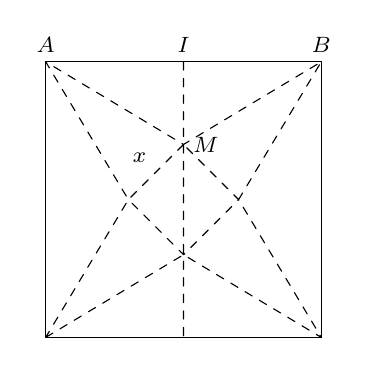
\begin{tikzpicture}[scale=0.7, font=\footnotesize, line join=round, line cap=round, >=stealth]
			\draw (0,0)--(5,0)--(5,5)--(0,5)--(0,0);
			\draw[dashed] (0,0)--(2.5,1.5)--(5,0)--(3.5,2.5)--(5,5)--(2.5,3.5)--(0,5)--(1.5,2.5)--(0,0) (2.5,3.5)--(1.5,2.5)--(2.5,1.5)--(3.5,2.5)--(2.5,3.5) (2.5,5)--(2.5,0);
			\node at (0,5) [above]{$A$};
			\node at (2.5,5) [above]{$I$};
			\node at (5,5) [above]{$B$};
			\node at (2.5,3.5) [right]{$M$};
			\node at (2,3) [above left]{$x$};
			\end{tikzpicture}
		}
		\noindent
		Ta có $y'=25\cdot 4x^3-25\sqrt{2}x^4=25x^3\left(4-\sqrt{2}x\right)$;\\
		Suy ra $y'=0\Leftrightarrow\hoac{&x=0\\&x=2\sqrt{2}.}$ \\
		Bảng biến thiên
		\begin{center}
			
\begin{tikzpicture}
			\tkzTabInit[nocadre=false,lgt=1.2,espcl=2.5,deltacl=0.6]
			{$x$ /0.6,$y'$ /0.6,$y$ /2}
			{$0$,$2\sqrt{2}$,$5\sqrt{2}$}
			\tkzTabLine{,+,$0$,-,}
			\tkzTabVar{-/, +/$320$,-/}
			\end{tikzpicture}
		\end{center}
		Vậy $\max\limits_{\left[0;5\sqrt{2}\right]} y=320$ tại $x=2\sqrt{2}$.\\
		Vậy mô hình có thể tích lớn nhất khi cạnh đáy bằng $2\sqrt{2}$.
	}
\end{ex}
\begin{ex}%[2D1K3-6]%Câu 10.
	Một trang chữ của một quyển sách tham khảo Văn học cần diện tích $384$ cm$^2$. Biết rằng trang giấy được canh lề trái là $2$ cm, lề phải là $2$ cm, lề trên $3$ cm và lề dưới là $3$ cm. Tìm chiều dài và chiều rộng của trang sách để trang sách có diện tích nhỏ nhất.
	\choice
	{Chiều dài bằng $32$ cm và chiều rộng bằng $12$ cm}
	{\True Chiều dài bằng $24$ cm và chiều rộng bằng $16$ cm}
	{Chiều dài bằng $40$ cm và chiều rộng bằng $20$ cm}
	{Chiều dài bằng $30$ cm và chiều rộng bằng $20$ cm}
	\loigiai{
		Gọi $x$, $y$ là chiều dài và chiều rộng của trang chữ.\\
		Theo đề bài ta có $xy=384$. Ta cần tìm $x$, $y$ sao cho $(x+4)(y+6)$ đạt giá trị nhỏ nhất.\\
		Ta có hàm $f(x)=xy+6x+4y+24=408+6x+4\cdot\dfrac{384}{x}=6x+\dfrac{1536}{x}+408\geq 2\cdot\sqrt{6\cdot 1536}=192$.\\
		Đẳng thức xảy ra khi $6x=\dfrac{1536}{x}\Leftrightarrow x=16\Rightarrow y=24$.\\
		Vậy với chiều dài là $24$ cm và chiều rộng là $16$ cm thì trang sách có diện tích nhỏ nhất.
	}
\end{ex}
\Closesolutionfile{ans}